\documentclass[12pt, oneside]{article}   
\usepackage{textcomp}

\usepackage{listings}
\lstset{language=R,literate={<-}{{$\gets$}}1}


\usepackage[a4paper,bindingoffset=0.2in,%
            left=0.75 in,right= 0.75 in,top= 0.75 in,bottom=0.75in,%
            footskip=.55in]{geometry}
                		
\geometry{letterpaper}                   		
\usepackage{amsmath}
\usepackage{graphicx}

\setlength{\parindent}{0pt}

\title{Bayesian Analysis of Randomized Controlled Trials}
\author{Julian Bautista, Alex Pavlakis, Advait Rajagopal}
%\date{\today}		
			
\begin{document}
\maketitle

\abstract{}	

\newpage 

\tableofcontents
\newpage

\section{Introduction}
Set up the paper.

\section{Bayesian Data Analysis}

\subsection{Model development}


\subsection{Model estimation}
Estimate the posterior distribution conditional on prior knowledge and the observed data.
\subsection{Posterior predictive checking}
Check the fit of the model and the resulting implications of the posterior parameter estimates.
\\
Repeat

\section{Comparison of Bayesian Data Analysis to Other Methods}
Write about the advantages of BDA over other formats.  How are they similar?  How are they different?

\section{Reproducibility}
Describe the philosophy and importance of reproducibility.  

Describe the steps of making research reproducible (e.g. sharing code, sharing data, explicitly specifying model, etc.)

\section{Impact of Smartphone App on Eating Behavior}

Hildebrandt et all (2017) conducted an experiment to test whether the Noom Monitor, a smartphone application, could augment the effect of in-person therapeutic treatment on binge eating behavior.  The treatment, known as \emph{guided self-help treatments based on cognitive-behavior therapy} (CBT-GSH), had been shown in previous research to reduce binge eating behavior by 10-50\%.  The Noom Monitor application was designed to facilitate CBT-GSH.  For this example, we consider two research questions from the experiment:
\begin{enumerate}
\item{Is CBT-GSH more effective at reducing binge eating behavior when facilitated by the Noom Monitor?}
\item{Does the effect of the Noom Monitor vary over time?}
\end{enumerate}

\subsection{Experimental design}

66 men and women with Bulimia Nervosa (BN) or Binge Eating Disorder (BED) were randomly assigned into two treatment conditions: CBT-GSH (N= 33) or CBT-GSH + Noom (N=33).  Therapy lasted for 12 weeks.  Assessments were conducted at weeks 0, 4, 8, 12, 24, and 36.  The primary outcome was Objective Bulimic Episodes (OBE).  

\subsection{Exploratory data analysis}

\begin{figure}
\centering
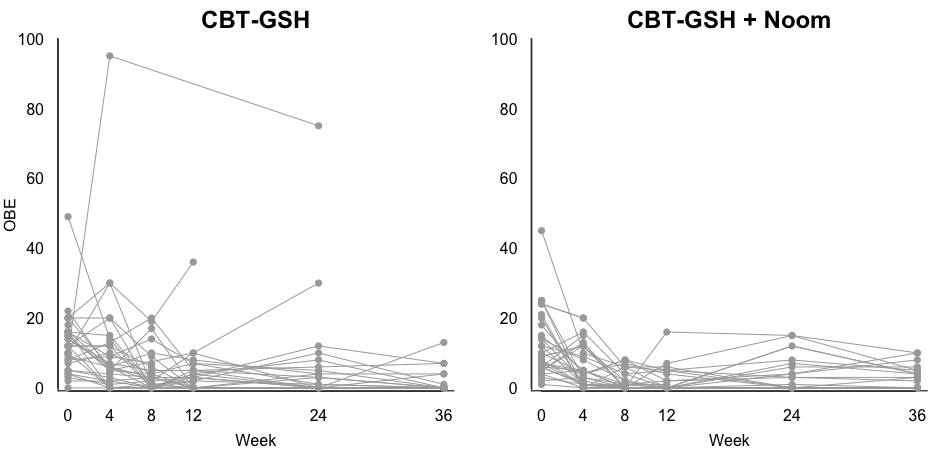
\includegraphics[width=\textwidth, height=\textheight, keepaspectratio]{Noom_paths.png}
\caption{\emph{Plots display OBEs over time for each individual in the CBT-GHS groups (left panel) and CBT-GHS + Noom group (right panel).}}
\end{figure}

Figure X displayes OBEs per week for each individual in both treatment conditions.  A few aspects of the data immediately stand out, which suggest that any model should account for individual-level effects and time-level effects, and should let treatment effects vary over time.  
\begin{itemize}
\item{The number of OBEs decreases over the course of the treatment for almost all subjects}
\item{The biggest decreases in OBEs appear to occur in the early stages of treatment}
\item{The primary sources of variation in OBE appear to be \emph{between people} and \emph{over time}.}
\end{itemize}

\newpage

\begin{figure}
\centering
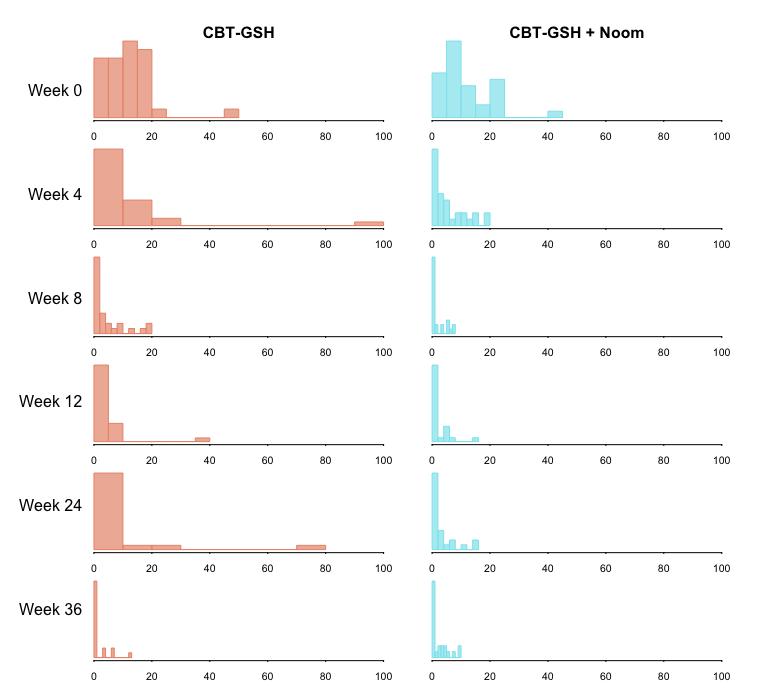
\includegraphics[width=\textwidth, height=\textheight, keepaspectratio]{noom_hist.png}
\caption{\emph{Histograms display the distribution of OBEs in each condition in each week.}}
\end{figure}

Figure Y displays the distribution of histograms in each condition in each week.  The distributions appear to condense around zero for both conditions over time, and the distributions in the CBT-GSH condition appear to have longer tails than those in the CBB-GSH+Noom condition.  

\subsection{Model development}

We analyze RCTs by modeling the outcome of interest (in this case OBE) as a function of the treatment and all available pre-treatment covariates.  The coefficients associated with the treatment reveal the average treatment effects.  Inclusion of all available pre-treatment covariates accounts for variation in the outcome variable, decreasing uncertainly around treatment effects and providing the model with more predictive power.  We conduct \emph{intent-to-treat} analysis, meaning that our inferences will be based on initial treatment assignment, and will not account for mid-experiment dropouts.  
\\

The outcome variable is restricted to be nonnegative integers, so we fit a Poisson regression model, with hierarchies on individuals, time periods, and treatment effects.  For each individual in each time period, the number of OBEs follows a Poisson distribution, with a mean dependent on the characteristics of the individual and the time period.  

\begin{align}
OBE_{i,t} &\sim Poisson(\lambda_{i,t}) \\
\lambda_{i,t} &= exp(\alpha_i + \beta_t + \gamma_tT_i + X_i\theta) \\
i &= 1, ..., 66 \\
t &= 0, 4, 8, 12, 24, 36 \\
T_i &=
    \begin{cases}
      0, & \text{if}\ CBT-GSH \\
      1, & \text{if}\ CBT-GSH + Noom \\
    \end{cases}
\end{align}

$\alpha$ is an individual-specific intercept, $\beta$ is a time-specific intercept, $\gamma$ is a time-specific treatment effect, $T$ is a treatment indicator, $X$ is a matrix of individual level covariates (age, sex, race, etc), and $\theta$ is a vector of individual level effects.
\\

We believe that individual-level intercepts are simultaneously unique to the individual and common to the population; that is, each individual has their own baseline predilection to engage in eating disorder behavior, but their baseline predilections are not drastically different from each other.  We operationalize this concept by modeling all individual-level intercepts as coming from a common distribution, with \emph{hyperparameters} $\mu_{\alpha}$ and $\tau_{\alpha}$.
\begin{align}
\alpha_i \sim Normal(\mu_{\alpha}, \tau_{\alpha}) \ \forall \ i \in 1,...,66
\end{align} 

Similarly, we believe that time-specific treatment effects may be unique to each period but similar over time. We operationalize this concept by modeling all time-specific treatment effects $\gamma$ as coming from a common distribution, with \emph{hyperparameters} $\mu_{\gamma}$ and $\tau_{\gamma}$.
\begin{align}
\gamma_t \sim Normal(\mu_{\gamma}, \tau_{\gamma}) \ \forall \ t \in 0, 4, 8, 12, 24, 36
\end{align} 

$\mu_{\gamma}$ is the \emph{grand mean}, the overall treatment effect; $\tau_{\gamma}$ is the variation in treatment effects over time; and each individual $\gamma_t$ is a time-period specific treatment effect.  This approach has a natural smoothing effect: any extreme estimates of $\gamma_t$ will be partially-pooled back toward the grand mean $\mu_{\gamma}$.
\\

To complete the model we must assign prior distributions to parameters (such as $\theta$) and hyperparameters (such as $\mu$).  These prior distributions will serve three main purposes:
\begin{enumerate}
\item{Transparency: priors allow us to be clear about our modeling assumptions.}
\item{Convergence: priors help the model "know where to look" and converge.}
\item{Inclusion of Additional Information: We usually have more information about an experiment than is represented by the data.  Priors allow us to include that information explicitly in our model.}
\end{enumerate}

For this model, we assign the following prior and hyperprior distributions:
\begin{align}
\mu_{\alpha} &\sim Normal(5, 5) \\
\tau_{\alpha} &\sim Cauchy^+(0, 30) \\
\mu_{\gamma} &\sim Normal(0, 5) \\
\tau_{\gamma} &\sim Cauchy^+(0, 30) \\
\theta &\sim Normal(0, 1) \\
\end{align}

The normal distributions around the individual and treatment effects allow us to guide the model to the appropriate range of parameter values, but with wide enough variance (5 in each case) to let the model find its own way in that range.  Half cauchy priors on the variance parameters are weakly informative, with much of their mass around zero but gentle slopes in their tails, which have been shown to be effective prior distributions for variance parameters (Gelman, 2006).

\subsection{Model estimation}
We estimate this model with \emph{Hamilton Monte-Carlo} in Stan.  Model code is appended to this document.  We find that the model converges with four chains of 2000 iterations each (see table M).  

\subsection{Posterior predictive checking}

\begin{figure}
\centering
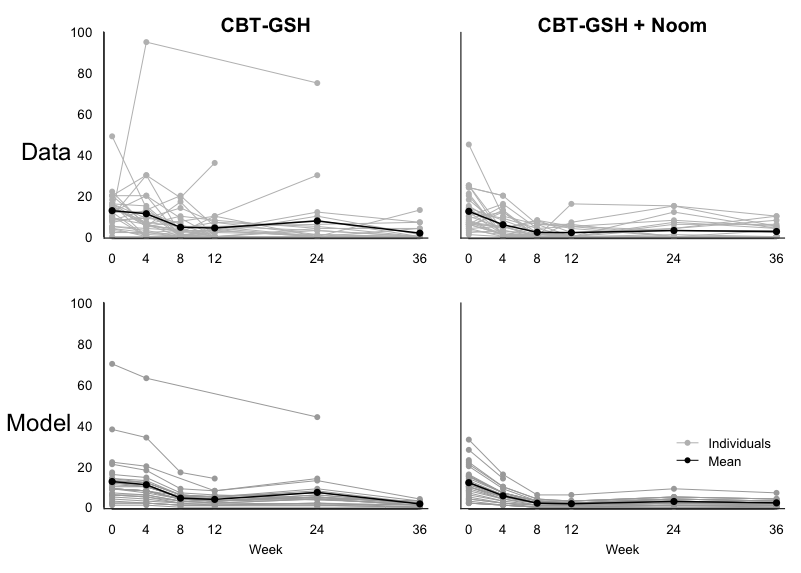
\includegraphics[width=\textwidth, height=\textheight, keepaspectratio]{ppc_sims.png}
\caption{\emph{Upper plots show OBEs in each period for each individual in both treatment group, with black lines representing means.  Lower plots show modeled OBEs for each individual in each treatment group, with black lines representing modeled means.  The model appears to be able to recover OBEs over time fairly well for both treatment conditions.}}
\end{figure}

Before using our model to make inferences about time-specific treatment effects, we check its fit by comparing model-simulated OBE to data OBE.  If model simulations do not track the data well, we may want to revisit our model's assumptions before trusting its inferences.  If the model's simulations recover patterns in the data, we are more inclined to trust its inferences.  
\\

Figure Q displays OBEs in each period for each individual in each treatment group, from raw data (upper plots) and model simulations (lowers plots).  Black lines display means for each.  This suggests that the model is broadly able to pick up on the key variables that determine OBE over time for the duration of this experiment.
\\

Another way to check the fit of the model is by comparing simulated data directly against the raw data.  Figure P shows this for both treatment conditions.  Simulated data for the Noom condition appears to better track the raw data than simulated data for the no Noom condition.  This is unsurprising, since the no Noom condition tended to have more outliers, which we would not expect (or want) our model to pick up perfectly from such a small sample.  
\\

\begin{figure}
\centering
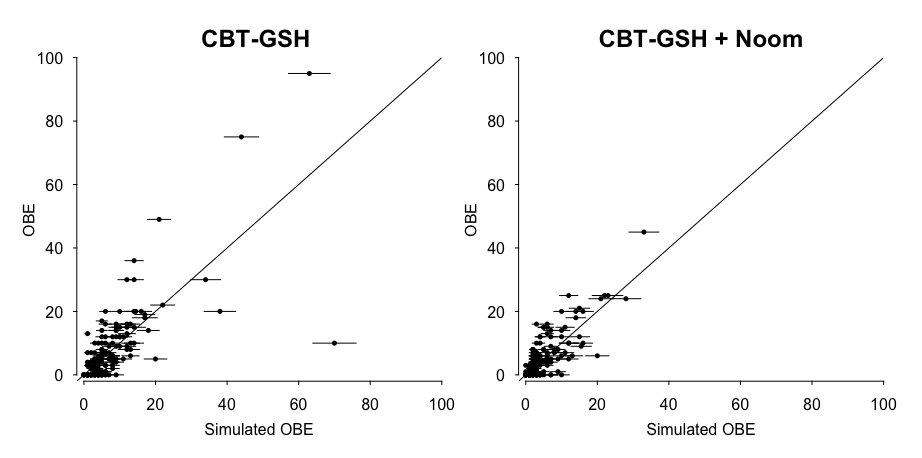
\includegraphics[width=\textwidth, height=\textheight, keepaspectratio]{obe_ppcs.png}
\caption{\emph{Plots display siulated OBEs to raw data for both treatment conditions.  Model simulations appear to match the raw data well, particularly for the Noom condition, which had fewer outliers.}}
\end{figure}

We conclude our model evaluations by mapping modeled density curves for each condition in each time period over the histograms in figure Y.  Figure BB shows that our model is able to broadly pick up on the patterns in the data over time and between treatment conditions.

\begin{figure}[h]
\centering
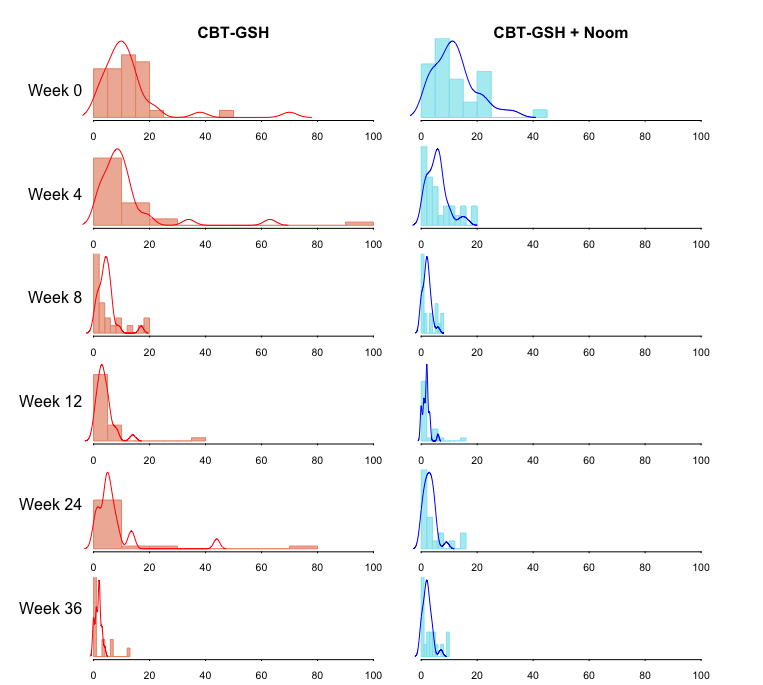
\includegraphics[width=\textwidth, height=\textheight, keepaspectratio]{ppc_hist_dens.png}
\caption{\emph{Histograms display the distribution of OBEs in each condition in each week.}}
\end{figure}

\subsection{Results}
Model results are displayed in table M.  Results suggest that using the Noom Monitor smartphone application during CBT-GSH may slightly decrease OBEs.  There some evidence that the treatment effect varies over time, with the Noom effect being slightly more pronounced during the later stages of therapy.
\\

Figure R displays modeled OBE for both treatment groups (upper plot) and smoothed treatment effects (lower plot).  In each measurement period, simulated OBE are higher for the No Noom condition than for the Noom condition, with some of the difference likely attributable to use of the Noom Monitor smartphone app.  

\begin{table}[t]
\centering
\begin{tabular}{r c c c c c}
  \hline
 & mean & 25\% & 50\% & 75\% \\ 
  \hline
  $\gamma_0$ & 0.18 & -0.45 & 0.15 & 0.78   \\ 
  $\gamma_4$ & -0.43 & -1.05 & -0.46 & 0.16   \\ 
  $\gamma_8$ & -0.70 & -1.33 & -0.71 & -0.10   \\  
  $\gamma_{12}$ & -0.65 & -1.28 & -0.68 & -0.04   \\  
  $\gamma_{24}$ & -0.72 & -1.34 & -0.75 & -0.11  \\  
  $\gamma_{36}$ & 0.21 & -0.42 & 0.19 & 0.82  \\ 
  \hline \hline
  $\mu_{\gamma}$ & -0.34 & -0.98 & -0.36 & 0.26  \\ 
  $\tau_{\gamma}$ & 0.64 & 0.43 & 0.56 & 0.77  \\ 
   \hline
\end{tabular}
\caption{\emph{Table displays model results for Noom effects in all six time periods and grand mean and variance parameters.}}
\end{table}


\begin{figure}[h]
\centering
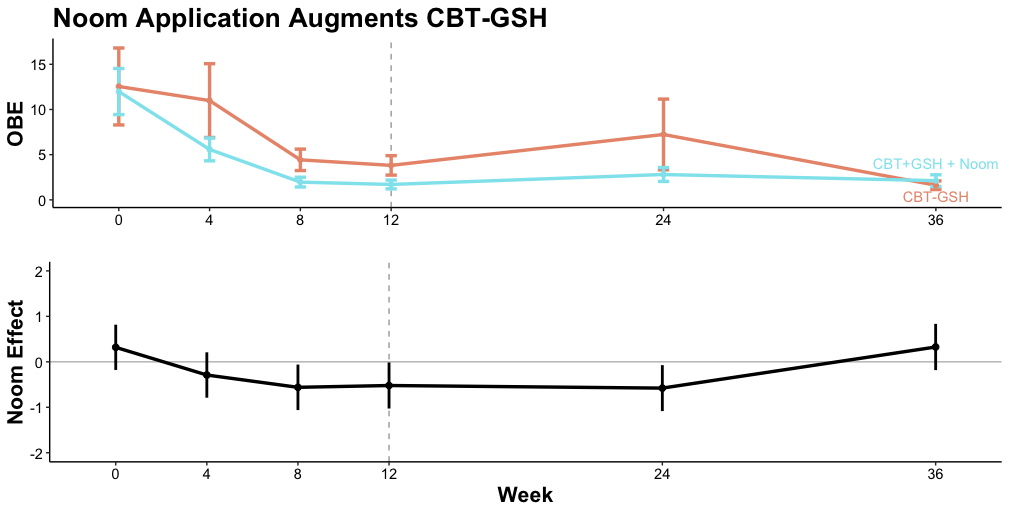
\includegraphics[width=\textwidth, height=\textheight, keepaspectratio]{noom_effect.png}
\caption{\emph{Upper plot displays modeled OBEs in each time period for the Noom (blue) and no Noom (orange) conditions with 95\% intervals.  Lower plot displays modeled treatment effects in each period,with 50\% intervals.}}
\end{figure}


\section{Conclusion}
So awesome

\section{Appendix}
All the math goes here

\end{document}